\documentclass[10pt,a4paper]{article}
\usepackage[margin=22mm]{geometry}
\usepackage[T1]{fontenc}
\usepackage{lmodern,amsmath,amssymb,booktabs,graphicx,microtype}
\usepackage[colorlinks=true,urlcolor=blue,citecolor=blue,linkcolor=blue]{hyperref}
\setlength{\parindent}{0pt}
\setlength{\parskip}{5pt}
\setlength{\belowcaptionskip}{5pt}
\newcommand{\PinnedOrder}{3.9979}
\newcommand{\SpringOrder}{3.9904}
\newcommand{\SpringLoad}{28.16771809}
\newcommand{\SpringGain}{2.85398}
\newcommand{\CoarsePercent}{0.2698}
\newcommand{\CoarseResidual}{6.123\times10^{-17}}
\newcommand{\BoundaryRows}{pinned & 9.86960440 & 9.86960567 & $1.290\times10^{-7}$ \\
clamped & 39.47841760 & 39.47849894 & $2.060\times10^{-6}$ \\
cantilever & 2.46740110 & 2.46740112 & $8.146\times10^{-9}$ \\
clamped-pinned & 20.19072856 & 20.19073945 & $5.393\times10^{-7}$ \\}
\newcommand{\ConvergenceRows}{0 & 4 & $5.121\times10^{-4}$ & $4.430\times10^{-4}$ & $6.503\times10^{-17}$ \\
0 & 8 & $3.277\times10^{-5}$ & $2.785\times10^{-5}$ & $6.113\times10^{-17}$ \\
0 & 16 & $2.060\times10^{-6}$ & $1.744\times10^{-6}$ & $2.521\times10^{-17}$ \\
0 & 32 & $1.290\times10^{-7}$ & $1.090\times10^{-7}$ & $4.553\times10^{-17}$ \\
10 & 4 & $2.698\times10^{-3}$ & $1.725\times10^{-3}$ & $6.123\times10^{-17}$ \\
10 & 8 & $1.895\times10^{-4}$ & $1.107\times10^{-4}$ & $9.413\times10^{-17}$ \\
10 & 16 & $1.217\times10^{-5}$ & $6.977\times10^{-6}$ & $5.794\times10^{-17}$ \\
10 & 32 & $7.655\times10^{-7}$ & $4.370\times10^{-7}$ & $8.086\times10^{-17}$ \\}

\title{BuckleMap: Rotational Restraint, Eigenvalue Error,\\
and Sensitivity in an Elastic Column}
\author{}
\date{Reproducible computational study, October 2026}
\begin{document}
\maketitle
\vspace{-7mm}
\begin{abstract}
Rotational end restraint can substantially increase an ideal elastic buckling
load, but a well-solved discrete eigenproblem alone does not establish an
accurate continuum prediction. This study implements exactly integrated cubic
Hermite elements in C++17, with Python assembly, analytical verification and
visualization. An independent scalar continuum equation tests equal end
springs, while four classical support conditions test constraint handling.
On nested meshes, the last measured load-convergence orders are \PinnedOrder\
for pinned ends and \SpringOrder\ for dimensionless spring stiffness ten.
At four elements, the latter case has \CoarsePercent\% load error despite a
normalized matrix residual of $\CoarseResidual$. Modal sensitivity agrees with
the continuum derivative and exhibits diminishing restraint benefit. These
results verify an ideal numerical model; they neither establish physical
validity nor provide safe design loads.
\end{abstract}

\section{Question, model and assumptions}
The question is how end restraint changes the first column eigenload, and how
to distinguish discretization error from algebraic solution error. Hermite
interpolation and linearized pre-buckling are established finite-element
concepts~\cite{hermite,nonlinear}; no new buckling theory is proposed here.
Consider a straight planar column of length $L$, positive rigidity $EI$,
and a uniform conservative compressive dead load $P$. The small bifurcation
displacement $w$ follows Euler--Bernoulli kinematics, $\theta=w'$; shear
deformation, material nonlinearity, imperfections and postbuckling are excluded.
Rotational end springs have stiffnesses $k_0,k_L\ge0$. The quadratic potential is
\begin{equation}
 \Pi_2(w)=\tfrac12\int_0^L EI(w'')^2\,dx
  +\tfrac12\sum_{s\in\{0,L\}}k_s w'(s)^2
  -\tfrac P2\int_0^L(w')^2\,dx.
\end{equation}
Its stationary weak form, for admissible test functions $v$, is
\begin{equation}
 a(w,v)=Pg(w,v),\quad a(w,v)=\int_0^L EI w''v''\,dx+\sum_s k_s w'(s)v'(s),
 \quad g(w,v)=\int_0^L w'v'\,dx. \label{eq:weak}
\end{equation}
The strong equation within each constant-rigidity segment is $EIw''''+Pw''=0$.
The units of $EI$ are force times length squared; those of $k_s$ are force
times length. Spring energy enters the elastic form, not the destabilizing
geometric form.

\section{Independent continuum reference}
For uniform rigidity, $w(0)=w(L)=0$ and equal springs, set $\kappa=k_s L/EI$
and $z=\sqrt{PL^2/EI}$. The symmetric first mode and its end conditions give
\begin{align}
 w(x)&=A\{\cos[z(x/L-1/2)]-\cos(z/2)\},\\
 \kappa\sin(z/2)+z\cos(z/2)&=0,\qquad \pi\le z\le2\pi. \label{eq:root}
\end{align}
In particular, $EIw''(0)=k_s w'(0)$ and $EIw''(L)=-k_s w'(L)$.
Brent's scalar root method yields $P=EI z^2/L^2$ independently of the FEM
matrices. The endpoints recover pinned $\pi^2EI/L^2$ and clamped
$4\pi^2EI/L^2$ loads. This derivation uses the classical column energy
model~\cite{stability}; it is a reference under the same physical assumptions,
not an independent physical experiment.

\newpage
\section{Discretization and implementation}
Each two-node element has DOFs $q_e=(w_1,\theta_1,w_2,\theta_2)^T$ and
cubic Hermite interpolation $w_h=Nq_e$. Exact integration gives
\begin{equation}
 K_e=\int EI(N'')^TN''\,dx,\qquad G_e=\int(N')^TN'\,dx,
 \qquad (K-PG)q=0. \label{eq:discrete}
\end{equation}
A dependency-free C++17 kernel supplies the element matrices through
pybind11. Python validates input, assembles both matrices, adds spring
stiffnesses to rotation diagonals, and eliminates constrained DOFs. The
congruence scaling $D_{ii}=K_{r,ii}^{-1/2}$ reduces mixed displacement/slope
conditioning. SciPy's symmetric definite eigensolver~\cite{scipy} solves
$(DK_rD)y=P(DG_rD)y$ and recovers $q_r=Dy$. The modes are $G$-orthonormal.
No penalty parameter is needed. Nonuniform meshes and elementwise constant
rigidity are supported, but the accuracy study uses uniform values.

For a simple first eigenvalue, differentiation with respect to equal springs
gives, at $L=EI=1$,
\begin{equation}
 \frac{dP_h}{d\kappa}=q^T\frac{dK}{d\kappa}q
 =\theta_0^2+\theta_L^2,\qquad q^TGq=1. \label{eq:sensitivity}
\end{equation}
The continuum derivative follows by implicit differentiation of
Eq.~\eqref{eq:root}, independently of the discrete eigenvectors.

\section{Verification setup and measured results}
All experiments use $L=EI=1$ and double precision. Convergence sequences use
$n=4,8,16,32$ elements at $\kappa=0$ and $10$. The restraint sweep uses $32$
elements and $\kappa=0$ plus $25$ logarithmically spaced values from $10^{-2}$
to $10^4$. Table~\ref{tab:boundary} checks four support presets. The
clamped--pinned reference is $z^2$, with $\tan z=z$, $z\in(4.4,4.6)$.
The cantilever is fixed at its left end. These cases exercise different
essential constraints and natural boundary conditions.

\begin{table}[h]
\centering\small
\caption{First loads on 32 elements. Errors concern the ideal continuum.}
\label{tab:boundary}
\begin{tabular}{lrrr}\toprule
Support & Continuum & FEM & Relative error\\\midrule
\BoundaryRows
\bottomrule\end{tabular}
\end{table}

Field error is the $L^2(0,1)$ difference after separately scaling analytical
and FEM symmetric modes to unit midpoint displacement; eight Gauss points per
element integrate its square. Algebraic error is measured on the original
reduced matrices:
\begin{equation}
 \eta=\frac{\|K_rq_r-P_hG_rq_r\|_\infty}
 {(\|K_r\|_\infty+P_h\|G_r\|_\infty)\|q_r\|_\infty}. \label{eq:residual}
\end{equation}
This normwise, scaling-dependent backward indicator is not an eigenvalue
forward-error bound. Table~\ref{tab:convergence} separates it from continuum
load and reconstructed-field error.

\begin{table}[h]
\centering\small
\caption{Mesh errors: $e_P=P_h/P-1$, unit-peak field error $e_w$,
and algebraic indicator $\eta$.}\label{tab:convergence}
\begin{tabular}{rrrrr}\toprule
$\kappa$ & $n$ & $e_P$ & $e_w$ & $\eta$\\\midrule
\ConvergenceRows
\bottomrule\end{tabular}
\end{table}

\newpage
\section{Restraint benefit and numerical interpretation}
Figure~\ref{fig:convergence} shows load and field convergence alongside the
matrix residual. Final load orders $\log_2(e_P(16)/e_P(32))$ are
\PinnedOrder\ and \SpringOrder. At $\kappa=10$, the 32-element load is
$\SpringLoad$; the continuum gain relative to pinned ends is $\SpringGain$.
The four-element spring case still has $\CoarsePercent\%$ load error at
$\eta=\CoarseResidual$. Increasing eigensolver precision would not remove
this discretization error.

\begin{figure}[h]
\centering
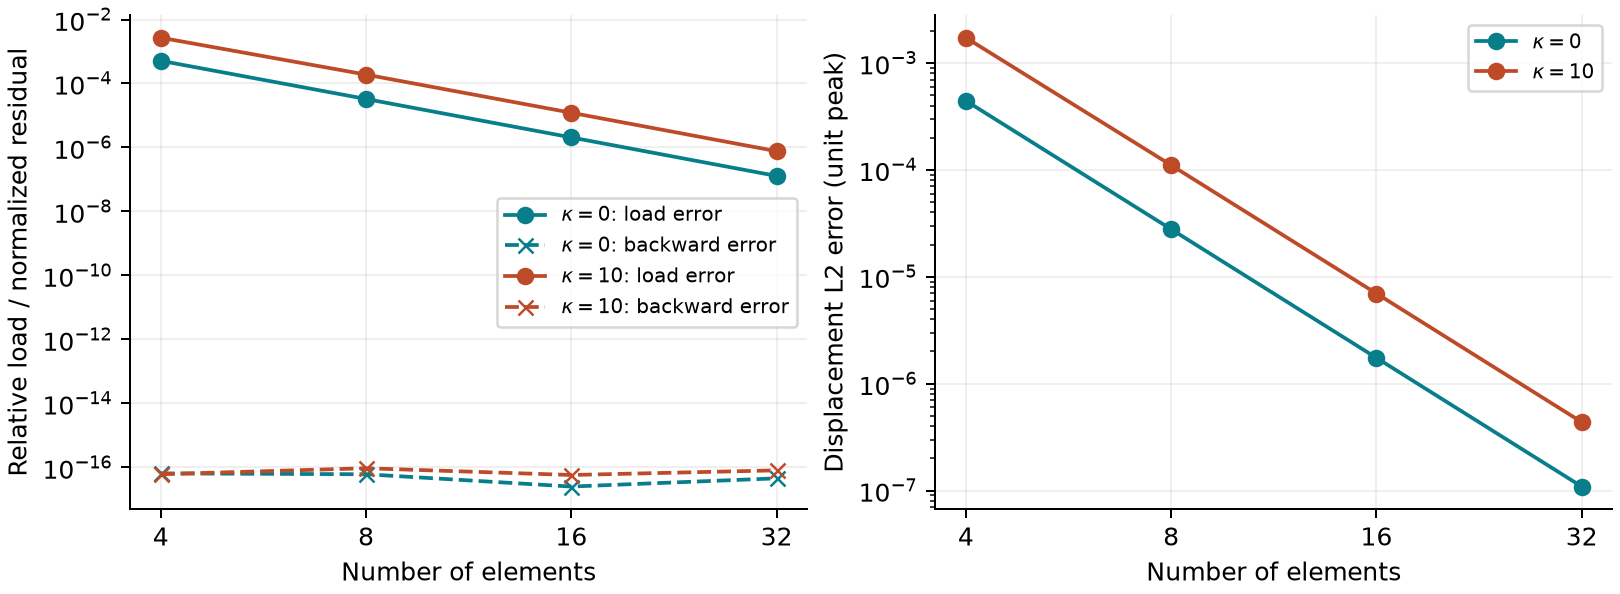
\includegraphics[width=\textwidth]{../examples/results/convergence.png}
\caption{Load versus algebraic error (left) and Hermite field error (right).
Curves are measured outputs; residuals depend on platform rounding.}
\label{fig:convergence}
\end{figure}

For conforming Hermite spaces and exact integration, the min--max principle
gives Ritz eigenvalues above ideal continuum values in exact arithmetic.
Nested refinement therefore decreases the first load toward the continuum
answer. The observed sequences are consistent with this property; the
floating-point implementation does not certify rigorous bounds. Field
reconstruction provides an additional check beyond a scalar eigenload.

\begin{figure}[h]
\centering
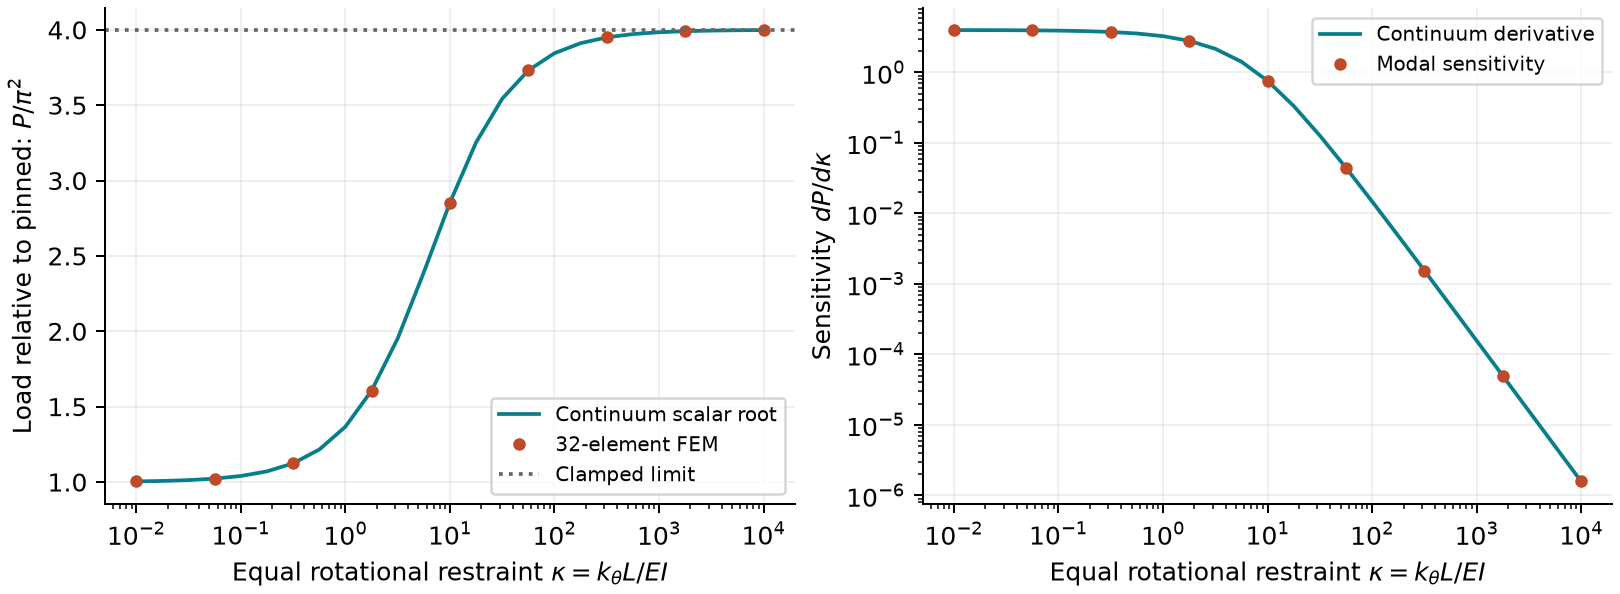
\includegraphics[width=\textwidth]{../examples/results/restraint.png}
\caption{Equal spring restraint raises the first load toward the clamped
limit, while sensitivity decreases. Curves use the continuum root and its
derivative; markers use the 32-element eigenproblem.}
\label{fig:restraint}
\end{figure}

The sensitivity agreement in Fig.~\ref{fig:restraint} supports the sign and
placement of spring contributions. Saturation follows Eq.~\eqref{eq:root};
it is not evidence that a real connection has a linear, load-independent
rotational stiffness. Equation~\eqref{eq:sensitivity} assumes a simple
eigenvalue; repeated eigenvalues require analysis of their invariant subspace.

\newpage
\section{Reproducibility and software checks}
The repository contains a native CMake/CTest target, an installable Python
package, CLI, and manuscript sources. The command
\texttt{bucklemap study --output output/study} regenerates the synthetic
measurements and figures. CSV and JSON retain unrounded values. The manuscript
builder derives every result table and numerical macro from the JSON. No
private data or course handouts are required. Topic-level course inspiration
is documented in the README; the code, figures and prose were authored for
this investigation.

The Python suite checks native matrices against independently fitted physical
polynomials and Gauss integration, cubic reconstruction, Euler references,
higher modes and geometric orthogonality, dimensional scaling, heterogeneous
nested refinement, spring monotonicity, modal derivatives against central
finite differences, invalid inputs and CLI behavior. Native checks exercise
rigid modes and symmetry. C++ warnings are errors; formatting checks cover both
languages. CI builds wheel and source distribution, tests the installed wheel
on Windows and Linux, and reproduces the numerical records. These are checks
of specified cases, not an exhaustive proof over permitted inputs.

The local environment uses Python 3.14 and MSVC 19.44; package versions are in
\texttt{requirements-tested.txt}. Cross-platform reproduction tolerances are
$3\times10^{-8}$ relative and $3\times10^{-10}$ absolute for ordinary numeric
fields, a $10^{-12}$ ceiling for $\eta$, and $0.02$ for derived convergence
orders. These allowances reflect BLAS-dependent rounding; they do not redefine
the continuum errors reported in Table~\ref{tab:convergence}.

The command \texttt{python paper/build.py --engine pdflatex} regenerates result
macros, compiles twice, rejects undefined references and overfull boxes, and
enforces a five-page maximum including references. Tectonic is also supported.
A SHA-256 manifest binds the PDF to source, solver files, data and figures.
CI renders all pages for inspection. Visual review is needed in addition to
automatic log and page-count checks. Identical PDF bytes across engines are
not required.

\section{Limitations and conclusion}
Dense storage is quadratic and the eigensolve cubic in the free-DOF count, so
the implementation targets small studies. Diagonal scaling reduces mixed-unit
conditioning problems but cannot guarantee accuracy for extreme mesh ratios,
restraint stiffnesses or rigidity contrasts. Only a uniform conservative
axial force is supported. Follower forces, shear flexibility, initial
crookedness, plasticity, nonlinear joints and load redistribution are excluded.
Agreement with the Euler model does not calibrate physical behavior; real
columns can fail below these ideal eigenloads. They must not be interpreted
as allowable loads or design-code compliance.

Within those assumptions, the experiments show diminishing benefit from
rotational restraint, nearly fourth-order load convergence on the tested
meshes, and agreement of modal and continuum sensitivities. They also show
why algebraic residual, discretization error and physical validity must be
assessed separately. BuckleMap is a reproducible implementation and
verification study of established mechanics, without claims of theoretical
novelty, affiliation or peer review.

\begin{thebibliography}{9}\small
\bibitem{hermite} TU Delft. \emph{Euler--Bernoulli beam elements}.
\href{https://teachbooks.tudelft.nl/computational-modelling/structural_linear/euler_bernouilli.html}{Finite Elements in Civil Engineering and Geosciences}, Sec.~4.1.
\bibitem{nonlinear} TU Delft. \emph{Geometrically nonlinear problems}.
\href{https://teachbooks.tudelft.nl/computational-modelling/solid_nonlinear/geometric_nonlinearity.html}{Finite Elements in Civil Engineering and Geosciences}, Sec.~5.4.
\bibitem{stability} TU Delft OpenCourseWare. \emph{Stability of Beams}.
\href{https://ocw.tudelft.nl/course-lectures/stability-of-beams/}{Buckling of Structures, lecture resource}.
\bibitem{scipy} SciPy developers. \emph{scipy.linalg.eigh}.
\href{https://docs.scipy.org/doc/scipy/reference/generated/scipy.linalg.eigh.html}{SciPy API reference}.
\end{thebibliography}
\end{document}
